\documentclass[aps,prl,onecolumn,superscriptaddress]{revtex4-2}

\usepackage{graphicx}
\usepackage{amsmath}
\usepackage{amssymb}

\begin{document}

\title{Supplementary Information for: Maximizing $\Delta_{\text{topo}}$ for Fault-Tolerant Topological Qubits}

\maketitle


\section{Supplementary Figures}

\begin{figure*}[t]
    \centering
    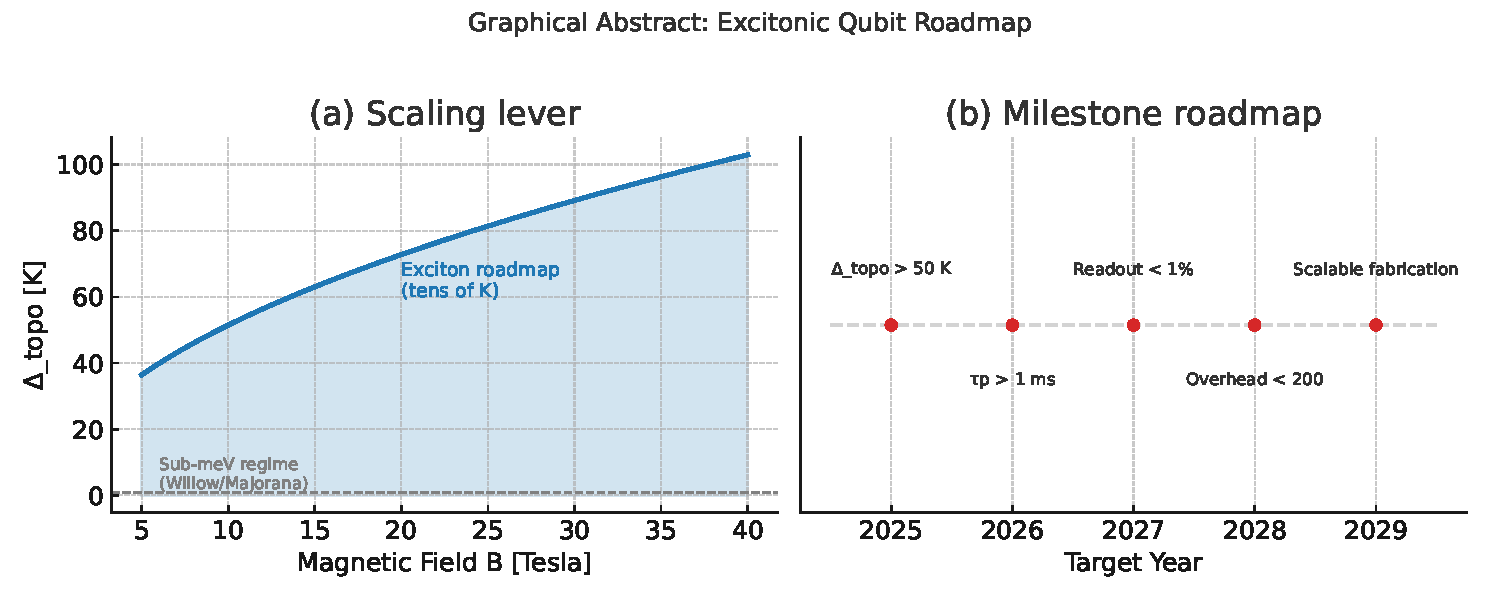
\includegraphics[width=0.95\textwidth]{figures/fig_graphical_abstract.pdf}
    \caption{Graphical Abstract: Excitonic Qubit Roadmap.
    (a) Scaling lever: the topological energy gap $\Delta_{\text{topo}}$ increases as $\propto \sqrt{B}/\epsilon$, enabling a transition from the sub-meV regime (superconducting and Majorana platforms) to the tens-of-Kelvin regime targeted by excitonic qubits. 
    (b) Milestone roadmap: five concrete targets are outlined from 2025 to 2029---demonstrating $\Delta_{\text{topo}} > 50$~K, parity lifetime $\tau_{p} > 1$~ms, parity readout error $<1\%$, logical overhead $<200$, and scalable fabrication. 
    Together these panels highlight both the physical lever and the stepwise experimental pathway toward intrinsically fault-tolerant excitonic qubits.}
    \label{fig:fig_graphical_abstract}
\end{figure*}

\begin{figure}[h]
    \centering
    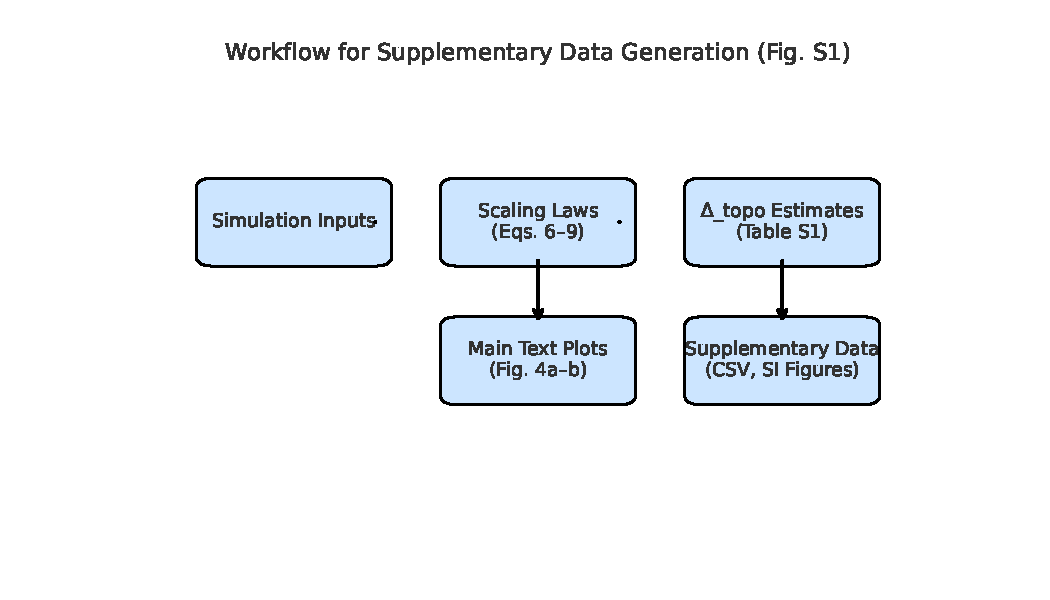
\includegraphics[width=0.85\linewidth]{supplementary/supplementary_fig1_workflow.pdf}
    \caption{Workflow for generating the supplementary data products. 
    Simulation inputs (magnetic field $B$, dielectric constant $\epsilon$, and scaling factor $\kappa$) are processed through the scaling laws defined in Eqs.~(6--9) of the main text, yielding numerical estimates of the topological gap $\Delta_{\text{topo}}$ (Table~S1). 
    These values are then visualized in the main text plots (Fig.~4a--b) and archived as machine-readable data (CSV). 
    The schematic illustrates how the supplementary resources directly support and extend the quantitative scaling analysis in Fig.~4.}
    \label{fig:workflow_supp}
\end{figure}




\section{Numerical Estimates of $\Delta_{\text{topo}}$}
To complement the scaling plots in Fig.~4 of the main text, we provide explicit numerical estimates of the topological energy gap $\Delta_{\text{topo}}$ as a function of magnetic field $B$, dielectric constant $\epsilon$, and scaling factor $\kappa$. 
The gap is evaluated using
\[
\Delta_{\text{topo}} \approx \kappa \frac{e^2}{4\pi \varepsilon_0 \epsilon \ell_B}, \qquad \ell_B = \sqrt{\frac{\hbar}{eB}}.
\]

Table~\ref{tab:delta_topo_estimates} reports representative values in Kelvin for $\epsilon = 4.0$ and $\kappa \in [0.05, 0.15]$. 
The full numerical dataset underlying this table and the main text Fig.~4 is provided as a machine-readable CSV file (\texttt{supplementary\_table1.csv}) included in the submission bundle.

\begin{table}[h]
\centering
\caption{Supplementary Table S1. Estimated topological gap $\Delta_{\text{topo}}$ in Kelvin for representative dielectric environment ($\epsilon=4.0$). Values computed using $\Delta_{\text{topo}} \approx \kappa e^2/(\epsilon \ell_B)$ with scaling factor $\kappa \in [0.05,0.15]$.}
\label{tab:delta_topo_estimates}
\begin{tabular}{lrrr}
\toprule
\textbf{B [T]} &  $\kappa=0.05$ &  $\kappa=0.10$ &  $\kappa=0.15$ \\
\midrule
10 &    25.7 &    51.5 &    77.2 \\
15 &    31.5 &    63.0 &    94.6 \\
20 &    36.4 &    72.8 &   109.2 \\
30 &    44.6 &    89.2 &   133.7 \\
45 &    54.6 &   109.2 &   163.8 \\
\bottomrule
\end{tabular}
\end{table}


\section{Supplementary Data}
The CSV file \texttt{supplementary\_table1.csv} contains the full numerical dataset of topological gap estimates $\Delta_{\text{topo}}$ as a function of magnetic field $B$, dielectric constant $\epsilon$, and scaling factor $\kappa$. 
These values underlie Supplementary Table~S1 and the scaling plots shown in Fig.~4 of the main text. 
Providing the machine-readable data ensures full reproducibility of the numerical results and allows readers to explore parameter ranges beyond those explicitly tabulated.

All supplementary figures, datasets, and plotting scripts are archived and openly available on Zenodo at \url{https://doi.org/10.5281/zenodo.17213190}.

\end{document}
